\documentclass[12pt,handout,ignorenonframetext,]{beamer}
\setbeamertemplate{caption}[numbered]
\setbeamertemplate{caption label separator}{: }
\setbeamercolor{caption name}{fg=normal text.fg}
\beamertemplatenavigationsymbolsempty
\usepackage{lmodern}
\usepackage{amssymb,amsmath}
\usepackage{ifxetex,ifluatex}
\usepackage{fixltx2e} % provides \textsubscript
\ifnum 0\ifxetex 1\fi\ifluatex 1\fi=0 % if pdftex
  \usepackage[T1]{fontenc}
  \usepackage[utf8]{inputenc}
\else % if luatex or xelatex
  \ifxetex
    \usepackage{mathspec}
  \else
    \usepackage{fontspec}
  \fi
  \defaultfontfeatures{Ligatures=TeX,Scale=MatchLowercase}
\fi
% use upquote if available, for straight quotes in verbatim environments
\IfFileExists{upquote.sty}{\usepackage{upquote}}{}
% use microtype if available
\IfFileExists{microtype.sty}{%
\usepackage{microtype}
\UseMicrotypeSet[protrusion]{basicmath} % disable protrusion for tt fonts
}{}
\newif\ifbibliography
\hypersetup{
            pdftitle={Développer un package R avec RStudio et git},
            pdfborder={0 0 0},
            breaklinks=true}
\urlstyle{same}  % don't use monospace font for urls
\usepackage{color}
\usepackage{fancyvrb}
\newcommand{\VerbBar}{|}
\newcommand{\VERB}{\Verb[commandchars=\\\{\}]}
\DefineVerbatimEnvironment{Highlighting}{Verbatim}{commandchars=\\\{\}}
% Add ',fontsize=\small' for more characters per line
\newenvironment{Shaded}{}{}
\newcommand{\KeywordTok}[1]{\textcolor[rgb]{0.00,0.00,1.00}{#1}}
\newcommand{\DataTypeTok}[1]{#1}
\newcommand{\DecValTok}[1]{#1}
\newcommand{\BaseNTok}[1]{#1}
\newcommand{\FloatTok}[1]{#1}
\newcommand{\ConstantTok}[1]{#1}
\newcommand{\CharTok}[1]{\textcolor[rgb]{0.00,0.50,0.50}{#1}}
\newcommand{\SpecialCharTok}[1]{\textcolor[rgb]{0.00,0.50,0.50}{#1}}
\newcommand{\StringTok}[1]{\textcolor[rgb]{0.00,0.50,0.50}{#1}}
\newcommand{\VerbatimStringTok}[1]{\textcolor[rgb]{0.00,0.50,0.50}{#1}}
\newcommand{\SpecialStringTok}[1]{\textcolor[rgb]{0.00,0.50,0.50}{#1}}
\newcommand{\ImportTok}[1]{#1}
\newcommand{\CommentTok}[1]{\textcolor[rgb]{0.00,0.50,0.00}{#1}}
\newcommand{\DocumentationTok}[1]{\textcolor[rgb]{0.00,0.50,0.00}{#1}}
\newcommand{\AnnotationTok}[1]{\textcolor[rgb]{0.00,0.50,0.00}{#1}}
\newcommand{\CommentVarTok}[1]{\textcolor[rgb]{0.00,0.50,0.00}{#1}}
\newcommand{\OtherTok}[1]{\textcolor[rgb]{1.00,0.25,0.00}{#1}}
\newcommand{\FunctionTok}[1]{#1}
\newcommand{\VariableTok}[1]{#1}
\newcommand{\ControlFlowTok}[1]{\textcolor[rgb]{0.00,0.00,1.00}{#1}}
\newcommand{\OperatorTok}[1]{#1}
\newcommand{\BuiltInTok}[1]{#1}
\newcommand{\ExtensionTok}[1]{#1}
\newcommand{\PreprocessorTok}[1]{\textcolor[rgb]{1.00,0.25,0.00}{#1}}
\newcommand{\AttributeTok}[1]{#1}
\newcommand{\RegionMarkerTok}[1]{#1}
\newcommand{\InformationTok}[1]{\textcolor[rgb]{0.00,0.50,0.00}{#1}}
\newcommand{\WarningTok}[1]{\textcolor[rgb]{0.00,0.50,0.00}{\textbf{#1}}}
\newcommand{\AlertTok}[1]{\textcolor[rgb]{1.00,0.00,0.00}{#1}}
\newcommand{\ErrorTok}[1]{\textcolor[rgb]{1.00,0.00,0.00}{\textbf{#1}}}
\newcommand{\NormalTok}[1]{#1}

% Prevent slide breaks in the middle of a paragraph:
\widowpenalties 1 10000
\raggedbottom

\AtBeginPart{
  \let\insertpartnumber\relax
  \let\partname\relax
  \frame{\partpage}
}
\AtBeginSection{
  \ifbibliography
  \else
    \let\insertsectionnumber\relax
    \let\sectionname\relax
    \frame{\sectionpage}
  \fi
}
\AtBeginSubsection{
  \let\insertsubsectionnumber\relax
  \let\subsectionname\relax
  \frame{\subsectionpage}
}

\setlength{\parindent}{0pt}
\setlength{\parskip}{6pt plus 2pt minus 1pt}
\setlength{\emergencystretch}{3em}  % prevent overfull lines
\providecommand{\tightlist}{%
  \setlength{\itemsep}{0pt}\setlength{\parskip}{0pt}}
\setcounter{secnumdepth}{0}
% Packages à charger
\usepackage[french]{babel}
\usepackage{lmodern}
\usepackage{graphicx}
\usepackage{xcolor}
\usepackage{textcomp} 
\usepackage{amsmath, amsfonts, amssymb, amsthm}
\usepackage{booktabs,multirow}
\usepackage{setspace}
\usepackage{float}
\usepackage{pgfpages}
\usepackage{colortbl}
\usepackage{epstopdf}
\usepackage{framed}
\usepackage{etoolbox}
\usepackage{tikz}


% Définition de couleurs utilisées par la suite
\definecolor{shadecolor}{RGB}{248,248,248}
\definecolor{grayInsee}{HTML}{5a5758}
\definecolor{redInsee}{HTML}{ed1443}

% Personnalisation du thème du beamer
\usetheme{default}
\setbeamertemplate{navigation symbols}{}
\setbeamertemplate{footline}[frame number]
\setbeamercolor{title}{fg=grayInsee}
\setbeamercolor{section in toc}{fg=redInsee}
\setbeamercolor{subsection in toc}{fg=grayInsee}
\setbeamertemplate{frametitle}{%
	\large \textcolor{grayInsee}{\subsecname}
	\\ \vspace{0.1cm} \Large \textcolor{redInsee}{\insertframetitle}
}
\setbeamercolor{local structure}{fg=redInsee}

% Instruction spécifiques à tikz
\usetikzlibrary{shapes,arrows,calc, positioning}
\tikzstyle{input} = [draw, rectangle,rounded corners, text width=2.5cm, fill=green!20, node distance=0.5cm, minimum height=2em, text centered]
\tikzstyle{output} = [draw, ellipse,fill=red!20, node distance=0.5cm, minimum height=2em, text centered]
\tikzstyle{block} = [rectangle, draw, fill=blue!20, 
    text width=1.5cm, text centered, minimum height=2em, node distance = 0.5cm]
\tikzstyle{line} = [draw, -latex', shorten >=2pt, shorten <=2pt]
\tikzset{
  invisible/.style={opacity=0},
  visible on/.style={alt={#1{}{invisible}}},
  alt/.code args={<#1>#2#3}{%
    \alt<#1>{\pgfkeysalso{#2}}{\pgfkeysalso{#3}} % \pgfkeysalso doesn't change the path
  },
}

% Personnalisation des débuts de partie et de sous-partie
\AtBeginSection[]{}
\AtBeginSubsection[]{}

% Affichage d'un fond gris derrière les exemples de code
\ifcsmacro{Shaded}{
  \renewenvironment{Shaded}{\begin{snugshade}}{\end{snugshade}}
}

\newcommand{\intertitre}[1]{\textbf{\textcolor{redInsee}{#1}}}

% Page de garde
\institute{
	
\includegraphics[height = 2.5cm]{Logo_Insee.png} \\ ~ \\ 
	\normalsize Martin \textsc{Chevalier} (DMS)}
\author{12 avril 2018}
\date{}

% Commande outil pour les exemples, etc.
\newcommand{\aparte}[2]{
	{\small\textsf{\textbf{#1} #2}}
}

\title{Développer un \emph{package} R \newline avec RStudio et git}
\date{}

\begin{document}
\frame{\titlepage}

\section{~}\label{section}

\subsection{~}\label{section-1}

\begin{frame}{Objectifs et plan de la présentation}

\begin{enumerate}
\def\labelenumi{\arabic{enumi}.}
\tightlist
\item
  Présenter les avantages du développement de \emph{packages} R pour un
  investissement méthodologique de moyen terme
\item
  \pause Introduire des concepts fondamentaux pour lancer le
  développement d'un \emph{package} R
\item
  \pause Faire un panorama des outils qui facilitent le développement
  collaboratif de \emph{packages} R
\end{enumerate}

\pause \bigskip \intertitre{Plan de la présentation}

\tableofcontents[currentsection, sectionstyle = hide, subsectionstyle = show/show/hide]

\end{frame}

\subsection{\texorpdfstring{Développer un \emph{package} R avec
RStudio}{Développer un package R avec RStudio}}\label{developper-un-package-r-avec-rstudio}

\begin{frame}{Qu'est-ce qu'un package R ?}

\intertitre{Définition} Ensemble de fonctions R documenté et structuré
de façon à être facilement réutilisé par d'autres.

\pause \bigskip \intertitre{Avantages}

\begin{itemize}
\tightlist
\item
  \vspace{-0.2cm} facile à utiliser pour d'autres utilisateurs (internes
  ou externes);
\item
  facile à publier pour les développeurs (numéro de version, etc.);
\item
  meilleure qualité : documentation, tests de chaque fonctionnalité
  (\og tests unitaires \fg{}), correction de bugs détectés par d'autres
  utilisateurs.
\end{itemize}

\pause \bigskip \intertitre{Inconvénients}

\begin{itemize}
\tightlist
\item
  \vspace{-0.2cm} plus complexe à développer que du code R standard ;
\item
  contraintes pour que le \emph{package} soit accepté sur le CRAN.
\end{itemize}

\end{frame}

\begin{frame}{Structure d'un \emph{package} R}

\begin{itemize}
\tightlist
\item
  nom unique (attention à la casse !);
\item
  \pause arborescence spécifique :
\end{itemize}

\pause \vspace{-0.3cm}

\begin{center}
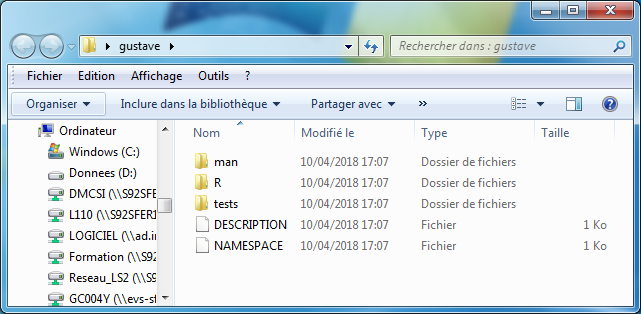
\includegraphics[height=5cm]{root_gustave.png}
\end{center}

\pause \intertitre{Références}
\href{https://cran.r-project.org/doc/manuals/r-release/R-exts.html}{\underline{Writing R Extensions}},
\href{http://r-pkgs.had.co.nz/}{\underline{R packages}},
\href{https://www.rstudio.com/wp-content/uploads/2015/03/devtools-cheatsheet.pdf}{\underline{\textit{cheatsheet}}}

\end{frame}

\begin{frame}[fragile]{Structure d'un \emph{package} R :
\texttt{DESCRIPTION}}

Le fichier DESCRIPTION est le fichier texte qui contient la plupart des
méta-données sur le \emph{package}:

\begin{itemize}
\tightlist
\item
  \pause son nom, son titre et une courte description;
\item
  \pause sa version (par exemple 0.2.9 pour gustave) et son mainteneur;
\item
  \pause les informations relatives à la propriété intellectuelle:
  licence, auteur, etc.;
\item
  \pause la version de R et la liste des \emph{packages} dont il dépend
  (mots-clés \texttt{Depends} et \texttt{Imports});
\item
  \pause d'autres informations techniques: encodage des fichiers, ordre
  dans lequel les fichiers R doivent être soumis (si nécessaire), etc.
\end{itemize}

\end{frame}

\begin{frame}[fragile]{Structure d'un \emph{package} R : \texttt{R/}}

Le dossier \texttt{R/} contient l'ensemble des codes R utilisés par le
\emph{package}, organisés comme le souhaite les développeurs.

\pause \bigskip Deux extrêmes :

\begin{itemize}
\tightlist
\item
  \pause \vspace{-0.3cm} toutes les fonctions du \emph{packages} dans le
  même fichier \texttt{.R};
\item
  \pause un fichier \texttt{.R} par fonction.
\end{itemize}

\pause \intertitre{Exemple de gustave}

\begin{center}
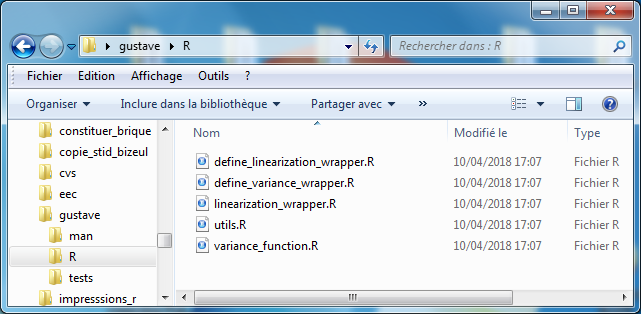
\includegraphics[height=3.5cm]{R_gustave.png}
\end{center}

\end{frame}

\begin{frame}[fragile]{\large Structure d'un \emph{package} R :
\texttt{man/} et \texttt{NAMESPACE}}

Le dossier \texttt{man/} contient l'ensemble des fichiers d'aide du
\emph{package} (un fichier par fonction).

\bigskip \pause Ces fichiers sont structurés par des balises et
permettent de générer le code HTML d'aide (accessible \emph{via}
\texttt{?}) ainsi que le manuel \texttt{.pdf} en ligne.

\pause \bigskip Le fichier \texttt{NAMESPACE} liste en particulier
l'ensemble des fonctions du \emph{package} qui ont vocation à être
accessibles aux utilisateurs.

\pause \intertitre{Remarque importante} Les fichiers du dossier
\texttt{man/} et le fichier \texttt{NAMESPACE} peuvent être générés
automatiquement par le \emph{package} roxygen2.

\end{frame}

\begin{frame}[fragile]{Structure d'un \emph{package} R :
\texttt{tests/}}

Le dossier \texttt{tests/} (optionnel) a vocation à contenir un ensemble
de tests qui vérifient le bon fonctionnement du \emph{package}.

\bigskip \pause On parle en particulier de \og test unitaire \fg{} pour
désigner le test d'une fonctionnalité précise (indépendamment des
autres).

\bigskip \pause Coder des tests unitaires nombreux qui sont relancés à
chaque évolution du \emph{package} permet de garantir la
\textbf{non-régression} entre les versions.

\bigskip \pause \intertitre{Remarque importante} Le \emph{package}
testthat offre un écosystème pour simplifier la mise en \oe uvre de
tests unitaires dans RStudio.

\end{frame}

\begin{frame}[fragile]{Structure d'un \emph{package} R : autres
dossiers}

Plusieurs autres dossiers optionnels peuvent être ajoutés à la racine
d'un \emph{package} R :

\begin{itemize}
\tightlist
\item
  \pause \texttt{data/}: il s'agit d'un dossier contenant des données
  (compressées) utilisées en particulier dans les exemples du
  \emph{package};
\item
  \pause \texttt{src/}: quand un \emph{package} fait appel à d'autres
  langages (C++ par exemple), le dossier \texttt{src/} contient le code
  source des fonctions en question (analogue au dossier \texttt{R/} mais
  pour les autre langages);
\item
  \pause \texttt{vignettes/} : le dossier \texttt{vignettes/} comporte
  le code (souvent au format Markdown, \texttt{.md}) des documents
  d'explication longs du \texttt{package}, qui sont nettement moins
  contraints que les éléments d'aide classiques (dans \texttt{man/}).
\end{itemize}

\end{frame}

\begin{frame}{Code source, compilation et installation}

L'arborescence décrite dans les diapositives précédentes est celle d'un
\emph{package} au moment de son développement, c'est-à-dire quand il est
à l'état de \textbf{code source}.

\pause \bigskip Pour être utilisé par R, un \emph{package} doit être
\textbf{compilé} et \textbf{installé} pour le système sur lequel R
s'exécute.

\pause \bigskip Quand un \emph{package} est \textbf{compilé}, il n'est
plus possible de lire directement le code des fonctions et le contenu de
l'aide.

\pause \bigskip \intertitre{Remarque importante}

\begin{itemize}
\tightlist
\item
  \pause sous Windows, en règle générale la compilation est faite par le
  CRAN en amont du téléchargement et de l'installation;
\item
  \pause sous Linux, l'installation est effectuée à partir du code
  source et le \emph{package} est compilé lors de l'installation.
\end{itemize}

\end{frame}

\begin{frame}{Utiliser RStudio pour développer un \emph{package}}

Le mode \og projet \fg{} de RStudio facilite considérablement le
développement de \emph{packages} R.

\pause L'ensemble des commandes complexes nécessaires pour produire un
\emph{package} est en effet accessible \emph{via} un \textbf{onglet
spécifique}.

\pause \vspace{-0.3cm}

\begin{center}
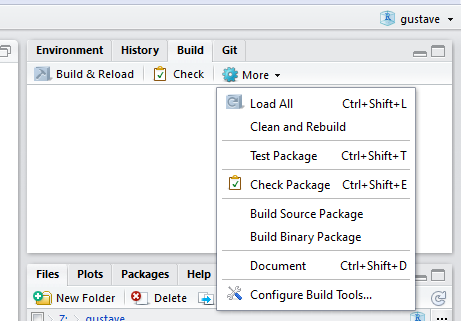
\includegraphics[height=4.2cm]{build_gustave.png}
\end{center}

\pause \vspace{-0.3cm}\intertitre{Remarque} Cette interface graphique
s'appuie notamment sur les \emph{packages} devtools, roxygen2 et
testthat.

\end{frame}

\begin{frame}[fragile]{Utiliser RStudio pour développer un
\emph{package}}

\begin{itemize}
\item
  \pause \og Load All \fg{} charge l'ensemble des fonctions du
  \emph{package};
\item
  \pause \bigskip \og Document \fg{} lance les fonctions de
  documentation automatique de roxygen2;
\item
  \og Test Package \fg{} lance les codes R du dossier \texttt{tests/},
  en particulier les tests conçus avec le \emph{package} testthat;
\item
  \pause \bigskip \og Build and Reload \fg{} réinstalle le
  \emph{package} et le lance;
\item
  \og Clean and Rebuild \fg{} supprime le \emph{package} et le
  réinstalle;
\item
  \og Build Source Package \fg{} et \og Build Binary Package \fg{}
  produisent un fichier \texttt{.tar.gz} facilement exportable, au
  format code source ou pré-compilé respectivement;
\item
  \pause \bigskip \og Check Package \fg{} vérifie que la structure du
  \emph{package} correspond (à peu près) à celle qui est attendue pour
  une mise en ligne sur le CRAN.
\end{itemize}

\end{frame}

\begin{frame}[fragile]{Documenter un \emph{package} avec roxygen2}

roxygen2 est un package qui permet d'\textbf{intégrer dans le même code
R} le code et la documentation d'une fonction.

\pause Concrètement, les éléments de documentation d'une fonction sont
intégrés dans le code \emph{via} des commentaires commençant par
\texttt{\#\textquotesingle{}} et structurés par un
\href{(https://cran.r-project.org/web/packages/roxygen2/vignettes/rd.html)}{\underline{ensemble de mots-clés}}
:

\footnotesize \pause

\begin{Shaded}
\begin{Highlighting}[]
\CommentTok{#' Ma super fonction}
\CommentTok{#' @description C'est une super fonction.}
\CommentTok{#' @param arg1 Un premier argument}
\CommentTok{#' @param arg2 Un deuxième argument}
\CommentTok{#' @examples ma_super_fonction()}
\CommentTok{#' @export ma_super_fonction}
\NormalTok{ma_super_fonction <-}\StringTok{ }\ControlFlowTok{function}\NormalTok{(arg1, arg2) }\StringTok{"Pouêt !"}
\end{Highlighting}
\end{Shaded}

\pause \normalsize \vspace{-0.2cm} roxygen2 parcourt les fichiers R du
dossier \texttt{R/} pour produire automatiquement les fichiers du
dossier \texttt{man/} ainsi que le fichier \texttt{NAMESPACE}.

\end{frame}

\begin{frame}[fragile]{Tester un \emph{package} avec testthat}

Le \emph{package} testthat fournit tout un ensemble de fonctions pour
\textbf{automatiser les tests} les fonctionnalités du \emph{package}
développé.

\pause \footnotesize

\begin{Shaded}
\begin{Highlighting}[]
\KeywordTok{context}\NormalTok{(}\StringTok{"Arithmétique"}\NormalTok{)}
\KeywordTok{test_that}\NormalTok{(}\StringTok{"les maths, ça marche !"}\NormalTok{, \{}
  \KeywordTok{expect_equal}\NormalTok{(}\DecValTok{2} \OperatorTok{+}\StringTok{ }\DecValTok{2}\NormalTok{, }\DecValTok{4}\NormalTok{)}
  \KeywordTok{expect_true}\NormalTok{(}\DecValTok{1} \OperatorTok{<}\StringTok{ }\DecValTok{2}\NormalTok{)}
  \KeywordTok{expect_error}\NormalTok{(}\DecValTok{1} \OperatorTok{*}\StringTok{ }\DecValTok{2}\NormalTok{, }\OtherTok{NA}\NormalTok{)}
\NormalTok{\})}
\end{Highlighting}
\end{Shaded}

\pause \normalsize \vspace{-0.2cm} Le résultat des tests menés est
compris par l'outil de vérification du \emph{package} (\og Check Package
\fg{}) ainsi que par l'interface de RStudio : dès qu'un test unitaire
échoue, il est identifié.

\pause Ce type de fonctionnalités pousse pour une systématisation des
tests unitaires dans le développement d'un \emph{package} (\emph{cf.}
\href{https://en.wikipedia.org/wiki/Test-driven_development}{\textit{\underline{test driven development}}}).

\end{frame}

\subsection{\texorpdfstring{Développer un \emph{package} R avec RStudio
et
git}{Développer un package R avec RStudio et git}}\label{developper-un-package-r-avec-rstudio-et-git}

\begin{frame}[fragile]{Qu'est-ce que git ?}

git est un des nombreux outils de gestion de version (\emph{version
control system} ou VCS en anglais) utilisé dans le monde du
développement logiciel.

\bigskip \pause Les outils de gestion de version (CVS, SVN par exemple)
ont été inventés pour répondre à \textbf{deux problèmes majeurs} :

\begin{itemize}
\item
  \pause la \textbf{conservation} de versions successives du code d'un
  projet : par défaut, les développeurs recourent à la technique du
  CPOLD (COPY + OLD), c'est-à-dire

  \pause \footnotesize

\begin{Shaded}
\begin{Highlighting}[]
\NormalTok{mon_code.R}
\NormalTok{mon_code_copie_}\FloatTok{1.}\NormalTok{R}
\NormalTok{mon_code_vdef.R}
\NormalTok{mon_code_180411_}\FloatTok{192600.}\NormalTok{R}
\end{Highlighting}
\end{Shaded}
\end{itemize}

\normalsize

\begin{itemize}
\tightlist
\item
  \pause \vspace{-0.3cm} la \textbf{collaboration} autour du même projet
  sans passer par le verrouillage de fichiers (exemple : fichier
  LibreOffice).
\end{itemize}

\end{frame}

\begin{frame}{Pourquoi développer un \emph{package} R avec git?}

\begin{enumerate}
\def\labelenumi{\arabic{enumi}.}
\item
  \textbf{Sécuriser} le code : conservation de l'ensemble des lignes de
  codes, même celles qui ne figurent plus dans la version actuelle du
  projet;
\item
  \bigskip \pause \textbf{Améliorer} la qualité du code : méta-donnée
  autour de chaque modification (donc suppression de commentaires
  superflus), relecture par d'autres facilitée ;
\item
  \bigskip \pause \textbf{Simplifier} la diffusion du \emph{package} :
  installation directe des \emph{packages} depuis un dépôt git (sans
  passer par le CRAN) ;
\item
  \bigskip \pause \textbf{Faciliter} la collaboration : travail en
  parallèle sur le code du \emph{package} puis consolidation des
  modifications.
\end{enumerate}

\bigskip \pause \intertitre{Référence}
\href{https://link.springer.com/book/10.1007\%2F978-1-4842-0076-6}{\underline{Pro Git}}
(Scott Chacon, Ben Straub)

\end{frame}

\begin{frame}[fragile]{En pratique : le répertoire (caché)
\texttt{.git/}}

Quand un projet est suivi en version par git, le répertoire (caché)
\texttt{.git} est ajouté à sa racine (on parle de dépôt git).

\bigskip \pause C'est dans ce répertoire \texttt{.git/} qu'est stockée
l'\textbf{ensemble de la mémoire du projet} : il est possible à partir
de ce seul dossier de récupérer toutes ses versions.

\bigskip \pause \intertitre{Remarque} Aucun \og serveur \fg{} n'est
nécessaire pour utiliser git en tant que tel, tout est contenu dans le
répertoire \texttt{.git/}.

\bigskip \pause Quand une modification est effectuée dans le projet, il
faut que celle-ci soit répercutée (\emph{via} les commandes de git) dans
le répertoire \texttt{.git/} pour être sauvegardée à jamais (ou presque
!).

\end{frame}

\begin{frame}{Une séance de travail avec git : RStudio}

Quand un projet RStudio est configuré pour utiliser, git, un onglet
supplémentaire apparaît :

Les principales fonctionnalités sont dans l'ordre : \og Diff \fg{},
\og Commit \fg{}, \og Pull \fg{}, \og Push \fg{} et enfin l'affichage de
l'historique des versions.

\end{frame}

\begin{frame}{Une séance de travail avec git : RStudio}

(historique des versions)

\end{frame}

\begin{frame}{Une séance de travail avec git : \emph{diff}}

Au début d'une séance de travail, en général aucun fichier n'apparaît
dans l'onglet git : les fichiers du projet correspondent exactement à la
dernière version du projet connue de git.

\bigskip \pause Au fur et à mesure que des changements sont faits, des
fichiers apparaissent avec une lettre à côté de leur nom:

\begin{itemize}
\tightlist
\item
  ``M'' pour les fichiers modifiés;
\item
  ``A'' pour les fichiers ajoutés;
\item
  ``D'' pour les fichiers supprimés.
\end{itemize}

\bigskip \pause À tout moment, le menu \og Diff \fg{} permet de vérifier
d'un coup d'oeil toutes les modifications effectuées.

\end{frame}

\begin{frame}{Une séance de travail avec git : \emph{diff}}

(diff)

\end{frame}

\begin{frame}[fragile]{\large Une séance de travail avec git :
\emph{stage} et \emph{commit}}

Les opérations \emph{stage} et \emph{commit} permettent de sauvegarder
les modifications effectuées dans git (i.e.~dans le répertoire
\texttt{.git} du projet).

\bigskip \pause Il est recommandé de les effectuer relativement
fréquemment : s'il s'avère nécessaire de revenir en arrière, il est
préférable qu'il y ait peu de changements depuis la dernière version.

\begin{enumerate}
\def\labelenumi{\arabic{enumi}.}
\tightlist
\item
  \bigskip \pause \textit{stage} : sélectionner les fichiers que l'on
  souhaite\ldots{}
\item
  \pause \textit{commit} : \ldots{}intégrer dans la mise à jour de la
  dernière version du projet dans git.
\end{enumerate}

\bigskip \pause \intertitre{Remarque} La plupart du temps, tous les
éléments ont vocation à être sélectionnés (\emph{staged}) pour le
prochain \emph{commit}.

\end{frame}

\begin{frame}{\large Une séance de travail avec git : \emph{stage} et
\emph{commit}}

(stage et commit)

\end{frame}

\begin{frame}{Une séance de travail avec git : \emph{bis repetita}}

\emph{diff}, \emph{stage} et \emph{commit} sont les trois opérations
essentielles à connaître pour travailler au quotidien avec git.

\bigskip \pause \intertitre{Remarque} Il est possible de corriger le
\emph{commit} précédent en cochant la case
\og \textit{Amend previous commit} \fg{}.

\bigskip \pause Elles aident à décomposer le travail en petites
opérations faciles à décrire et à valider individuellement.

\bigskip \pause \intertitre{Exemple} Pour développer une nouvelle
fonctionnalité:

\begin{enumerate}
\def\labelenumi{\arabic{enumi}.}
\tightlist
\item
  Écrire le test qui correspond au résultat souhaité
\item
  Écrire une première version minimale de la fonctionnalité
\item
  Écrire une version plus complète de la fonctionnalité
\end{enumerate}

\end{frame}

\begin{frame}[fragile]{\large git : un outil de gestion de version
décentralisé}

Jusqu'à présent, toutes les opérations ont été faites dans le dossier
personnel d'un développeur en particulier.

\bigskip \pause Pour collaborer avec d'autres développeurs sur le même
projet, il suffit que les dossiers \texttt{.git/} des uns et des autres
\textbf{s'échangent l'histoire du projet}.

\bigskip \pause La principale innovation de git est d'être
\textbf{complètement décentralisé} : le développement pourrait ne
s'appuyer que sur des échanges \og de pair-à-pair \fg{} entre
développeurs.

\bigskip \pause En pratique cependant, un dépôt particulier est choisi
comme dépôt de référence : même si on l'appelle en général le
\og serveur \fg{}, il ne présente \textbf{aucune particularité
technique}.

\end{frame}

\begin{frame}{Collaborer avec git : \emph{remote}}

L'opération \emph{remote} permet d'ajouter et de configurer de nouveaux
dépôts avec lesquels le dépôt local est susceptible d'échanger.

\bigskip \pause \intertitre{Remarque} Les dépôts en question peuvent
être distants ou sur la même machine que le dépôt local (par exemple sur
un espace partagé sur AUS).

\bigskip \pause Concrètement, cette opération permet d'associer un nom
symbolique aux dépôts distants.

\bigskip \pause \intertitre{Exemple} Le dépôt
\url{https://github.com/martinchevalier/gustave} est le dépôt distant
libellé ``github'' du dépôt git ``gustave'' de mon poste de travail.

\end{frame}

\begin{frame}{Collaborer avec git : \emph{pull} et \emph{push}}

L'opération \emph{pull} permet de mettre à jour le dépôt local à partir
du contenu d'un dépôt distant.

\bigskip \pause Dans le cadre d'un travail coopératif, cette opération a
vocation à être effectuée \textbf{en début de séance de travail}.

\bigskip \pause Inversement, l'opération ush permet de mettre à jour un
dépôt distant à partir du contenu du dépôt local.

\bigskip \pause Dans le cadre d'un travail coopératif, cette opération a
vocation à être effectuée \textbf{en fin de séance de travail}.

\end{frame}

\begin{frame}{Collaborer avec git : conflits}

Il peut survenir (en général à l'occasion d'un \emph{push}) que git ne
parvienne pas à synchroniser les deux dépôts automatiquement.

\bigskip \pause Cela survient en général quand des modifications ont été
effectuées en parallèle sur les mêmes lignes de code.

\bigskip \pause Dans cette situation, il est impératif de régler les
conflits pour finaliser l'opération :

\begin{itemize}
\tightlist
\item
  les zones en conflit sont indiquées spécifiquement par git;
\item
  le développeur modifie l'ensemble des zones en conflit, teste sa
  solution et propose un commit de fusion (\emph{merge}).
\end{itemize}

\end{frame}

\begin{frame}{Collaborer avec git : branches}

C'est la manière dont git permet de construire des dérivations (ou
\og branches \fg{}) par rapport à la ligne de développement principal
qui est la principale raison de son succès.

\bigskip \pause \intertitre{Exemple} Pour développer une fonctionnalité
complexe sur plusieurs semaines, un développeur a le choix entre:

\begin{itemize}
\tightlist
\item
  \pause effectuer des \emph{push} chaque jour : déstabilisation de
  l'ensemble du programme (car la fonctionnalité ne sera pas
  complètement codée);
\item
  \pause effectuer un seul \emph{push} à la fin : pas de relecture par
  les pairs, gros travail de fusion à effectuer.
\end{itemize}

\bigskip \pause  Dans cette situation, créer une nouvelle branche permet
de poursuivre un développement \textbf{sans perturber la branche
principale} et tout en intégrant ses évolutions.

\end{frame}

\begin{frame}{Collaborer avec git : plateformes}

De nombreuses plateformes se sont construites autour de git pour
faciliter le travail des développeurs : github.com, serveur web libre
gitlab.

\bigskip \pause Leur fonction première est d'être un candidat naturel
pour accueillir le \textbf{dépôt de référence des projets}.

\bigskip \pause Elles comportent néanmoins un certain nombre de
\textbf{fonctions annexes très appréciables}:

\begin{itemize}
\tightlist
\item
  \pause exploration et modification du code source des projets dans un
  navigateur web;
\item
  \pause centralisation des rapports de bugs, documentation;
\item
  \pause couche sociale permettant la collaboration entre développeurs;
\item
  \pause tests et déploiement automatique.
\end{itemize}

\end{frame}

\end{document}
